\par
In this chapter, I report the summer 2023 internship work at LBNL and additional numerical implementations I continued to finish this thesis.

As we mentioned in Chapter \ref{sec:intro_complex_fluid}, we consider the stress tensor of the form as in equation (\ref{eq_CN_tau}), 
\begin{equation}
  \boldsymbol{\tau} =
  \nu_0  \bm{A}_1 +  \nu_1  \bm{A}_1^2 + \nu_2 \bm{A}_2 ,
\nonumber
\end{equation}
to solve an incompressible flow with the Navier-Stokes equation,
\begin{align}
  \nabla \cdot \vec{u} = 0 
  \nonumber \\
  \rho 
  \left( 
     \frac{\partial \vec{u}}{\partial t} + \vec{u}\cdot \nabla \vec{u}
  \right)
  + \nabla P 
    = \nabla \cdot   \bm{\tau} 
    +  \rho  \vec{g} ,
  \nonumber
  \end{align}
in which  they were introduced in Chapter 1; equations (\ref{eq_conserv_mass}) and (\ref{eq_momentum_NS}).
In the AMReX-incflo code, three ways of time integration methods are implemented to update the velocity and pressure. Among them, we can only use the explicit Euler scheme since we have a $\bm{\tau}$ having a quadratic relationship with the strain rate $\bm{D}$, which is a function of the velocity $\vec{u}$. 
We re-write the momentum equation by splitting the deviatoric stress tensor, ${\bm \tau}$, into two parts, 
\[
 {\bm \tau}= {\bm \tau_1} + {\bm \tau_2},
\] 
where ${\bm \tau_1}$ and ${\bm \tau_2}$ are the linear and quadratic effects in terms of strain rate, ${\bm D}$, of the deviatoric stress tensor, i.e., 
\[
  {\boldsymbol \tau_1} \propto \boldsymbol{D}
  \ \ \ \ \ \text{and}
   \ \ \ \ \ 
{\boldsymbol \tau_2} \propto {\boldsymbol D^2}.
\]
\section{Divergence of the econd-order strain rate stress tensor}
Why do we need the 'divtau'? how is this connected? 
-> need to explain the Navier stokes first. 
In the AMReX library, the linear shear stress tensor computation is already implemented. For the higher-order term,
\[
  {\bm \tau}_{2} = 
  \tilde{\eta}_2
  \left( {\bm D}^2  - \frac{\text{tr}\left({\bm D}^2\right)}{3}{\bm I} \right)
  + \tilde{\eta_3} 
  \biggl( {\bm{DW}} - {\bm{WD}} \biggr)  
\]
we needed to create a new operator to compute $ {\bm \tau}_{2}$. Moreover, the divergence of it, $\nabla \cdot {\bm \tau}_{2}$, is required to solve for velocity. Note that 
\[
\tilde{\mu_2} =  \mu_2  \dot{\gamma}^2
+  \kappa_2 
\ \ \ \ \ \text{and} \ \ \ \ \ \
\tilde{\eta_3} =    \eta_3 \dot{\gamma}^2 .
\]
We use Mathematica to find the exact component of  ${\bm D}^2 - (\text{tr}({\bm D}^2)/3) {\bm I} = \left[ D_1  \ D_2 \ D_3 \right]$:
\\
First column:
\[
D_1 =
\begin{bmatrix}
   \frac{1}{3} \left(\left(u_y+v_x\right)^2+\left(u_z+w_x\right)^2+8 u_x^2-2 \left(v_z+w_y\right)^2-4 v_y^2-4 w_z^2\right)
   \\
   \left(u_z+w_x\right) \left(v_z+w_y\right)+2 \left(u_x+v_y\right) \left(u_y+v_x\right)
   \\
   \left(u_y+v_x\right) \left(v_z+w_y\right)+2 \left(u_x+w_z\right) \left(u_z+w_x\right)
\end{bmatrix}
\]
Second column:
\[
D_2 = 
\begin{bmatrix}
   \left(u_z+w_x\right) \left(v_z+w_y\right)+2 \left(u_x+v_y\right) \left(u_y+v_x\right)
   \\
   \frac{1}{3} \left(\left(u_y+v_x\right)^2-2 \left(u_z+w_x\right)^2-4 u_x^2+\left(v_z+w_y\right)^2+8 v_y^2-4 w_z^2\right)
   \\
   \left(u_y+v_x\right) \left(u_z+w_x\right)+2 \left(v_y+w_z\right) \left(v_z+w_y\right)
\end{bmatrix}
\]
Third one:
\[
D_3 = 
\begin{bmatrix}
   \left(u_y+v_x\right) \left(v_z+w_y\right)+2 \left(u_x+w_z\right) \left(u_z+w_x\right),
    \\
   \left(u_y+v_x\right) \left(u_z+w_x\right)+2 \left(v_y+w_z\right) \left(v_z+w_y\right),
   \\
   \frac{1}{3} \left(-2 \left(\left(u_y+v_x\right)^2+2 \left(u_x^2+v_y^2\right)\right)+\left(u_z+w_x\right)^2+\left(v_z+w_y\right)^2+8 w_z^2\right)
\end{bmatrix}
\]
We also can write each column of ${\bm{DW}} - {\bm{WD}} = \left[ DW_1 \ DW_2 \ DW_3  \right]$:
\\
First column:
\[
DW_1 = 
\begin{bmatrix}
    2 \left(- u_{y}^2-u_{z}^2  + v_{x}^2 + w_{x}^2\right)
    \\
    -2 \left(u_{z} v_{z}+\left(v_{y}-u_{x}\right) \left(u_{y}-v_{x}\right)-w_{y} w_{x}\right)
    \\
    -2 
    \left(
    u_{y} w_{y}+ \left(w_{z}-u_{x}\right) \left(u_{z}-w_{x}\right)- v_{z} v_{x}
    \right)
\end{bmatrix}
\]
Second column:
\[
DW_1 = 
\begin{bmatrix}
    -2 \left(u_{z} v_{z}+\left(v_{y}-u_{x}\right) \left(u_{y}-v_{x}\right)-w_{y} w_{x}\right)
    \\
    2 \left(- v_{x}^2 - v_{z}^2 +u_{y}^2 + w_{y}^2\right)
    \\
    -2 
    \left(
    -u_{z} u_{y}+ \left(w_{z}-v_{y}\right) \left(v_{z}-w_{y}\right)+ v_{x} w_{x}
    \right)
\end{bmatrix}
\]
Third column:
\[
DW_1 = 
\begin{bmatrix}
   -2 u_{y} w_{y}-2 \left(w_{z}-u_{x}\right) \left(u_{z}-w_{x}\right)+2 v_{z} v_{x}
   \\
   2 u_{z} u_{y}-2 \left(w_{z}-v_{y}\right) \left(v_{z}-w_{y}\right)-2 v_{x} w_{x}
   \\
   2 \left(u_{z}^2+v_{z}^2-w_{y}^2-w_{x}^2\right)
\end{bmatrix}
\]
For now, we compute each stress term separately and assemble them when we need to use them. We might want to explore other ways to process these steps more efficiently. 
\section{Numerical implementation for a time integral}
\section{Explicit Runge-Kutta 2 (RK2) method}
What do you have here?
\section{Predictor-Corrector method}
This is the same idea as the 2-stage Runge-Kutta method. We denote the advection term, ${\bm u} \cdot \nabla {\bm u}$ as ${\bm A}$. 
\\
$<${\bf Predictor}$>$
\\
First, consider the non-linear stress tensor, ${\bm \tau_2}$ as a force term, and solve for the first predictor values, that are ${\bm u}^*$ and ${\bm u}^*$:
\[
\frac{{\color{blue}{\bm u}^*} - {\bm u}^n}{\Delta t} 
+  {\bm A}^{n+1/2} 
=- \frac{1}{\rho}  \biggl(
\frac{\nabla \cdot {\color{blue}{\bm \tau}_1^*} + \nabla \cdot{\bm \tau}_1^n}{2} 
+ \nabla \cdot {\bm \tau}_2^n 
- \nabla p^n
+{\bm g}
\biggr)
\]
We solve for blue terms - 
\[
{\color{blue}{\bm u}^*} +
\frac{1}{\rho} 
\left( 
\frac{\nabla \cdot {\color{blue}{\bm \tau}_1^*}}{2}
\right)
=
{\bm u}^n
- {\bm A}^{n+1/2} \Delta t
- \frac{\Delta t}{\rho} \biggl(
\frac{ \nabla \cdot{\bm \tau}_1^n}{2} 
+ \nabla \cdot {\bm \tau}_2^n 
- \nabla p^n
+{\bm g}
\biggr)
\]
\\
$<${\bf Corrector}$>$
\\
Once we obtain the predictor (star) velocity, we use it to compute the second order stress tensor, ${\bm \tau}_2^*$.
\[
\frac{{\color{red}{\bm u}^{n+1}} - {\bm u}^n}{\Delta t} 
+  {\bm A}^{n+1/2} 
=- \frac{1}{\rho}  \biggl(
\frac{\nabla \cdot {\color{red}{\bm \tau}_1^{n+1}} + \nabla \cdot{\bm \tau}_1^n}{2} 
+ \frac{\nabla \cdot {\bm \tau}_2^{n} + \nabla \cdot {\color{blue}{\bm \tau}_2^*}}{2} 
- \nabla p^n
\biggr)
\]

Now, we need to solve for red - next time step values:
\[
{\color{red}{\bm u}^{n+1}} 
+\frac{1}{\rho} 
\left(
\frac{\nabla \cdot {\color{red}{\bm \tau}_1^{n+1}}}{2}
\right)
=
{\bm u}^n 
 -{\bm A}^{n+1/2} \Delta t
- \frac{\Delta t}{\rho}  \biggl(
\frac{ \nabla \cdot{\bm \tau}_1^n}{2} 
+ \frac{\nabla \cdot {\bm \tau}_2^{n} + \nabla \cdot {\color{blue}{\bm \tau}_2^*}}{2} 
- \nabla p^n
\biggr)
\]
Note that ${\bm \tau}_i^* = {\bm \tau}({\bm u}^*, \eta_i)$.
\section{Validation}
\begin{itemize}
  \item We follow the experiment setup found in \cite{couturier_suspensions_2011}
  \item We want to present the N1 and N2 values with various volume fractions: from 0.1 to 0.5.
  \item the geometry of a tilted trough with rigid spheres in a Newtonian fluid. 
\end{itemize}
\section{Granular rheology}
We recall the stress tensor for the fluid momentum equation, introduced in Chapter 1, for a non-Newtonian fluid:
\begin{align}
  \bar{\bar{\sigma}}
    = -P \bar{\bar{I}}  + \mu(\dot{\gamma}) {\bm D}.
  \end{align}
{\color{red}WARNING: NOTATIONS}
\\
In this section, we explain the details of the methodology to compute granular flow velocity when external pressure is present. We introduce a stress tensor with a higher-order strain rate that can describe non-isotropic flow effects. A new apparent viscosity computation using the well-known $\mu(I)$ relation can also be found [{\color{blue}REFERENCE}]. With the new deviatoric stress tensor, we solve for incompressible granular flow using incflo. 
\begin{figure}[ht]
  \begin{center}
    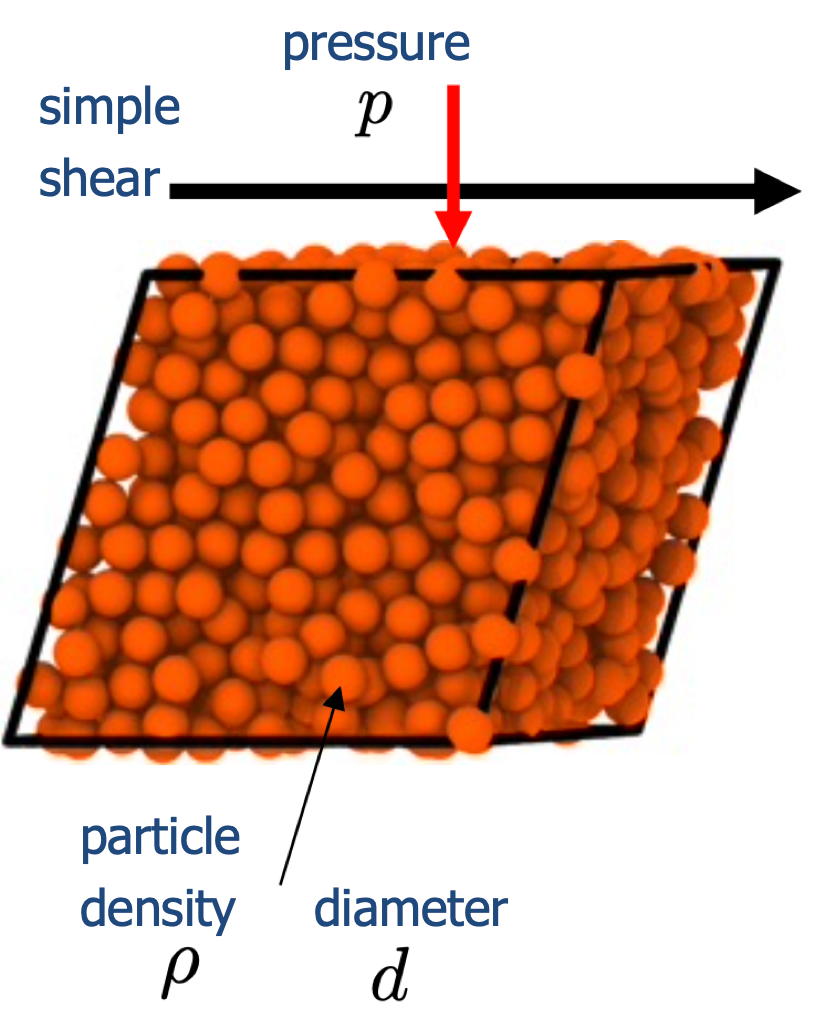
\includegraphics[scale=0.4]{figures/fig_granular_ex.png}
    \end{center}
  \caption{Schematics of granular flow in a box with external pressure.({\color{red}Citation})}
  \label{fig_Laminar_shear}
\end{figure}

To describe a non-isotropic flow, we consider the Cauchy stress tensor, $\bar{\bar{\sigma}}$, up to the second order of strain rate \cite{srivastava_viscometric_2021}. In particular, we see the deviatoric tensor, $\bar{\bar{\sigma}} - P \bar{\bar{I}}$, as 
% \begin{align*}
% \bar{\bar{\sigma}} - P {\bm I} \equiv
%   {\bm {\bm \tau}}
%   =  \ \mu_1 {\bm D} 
%   + \mu_2  \left[ {\bm D}^2  - \frac{\text{tr}\left({\bm D}^2\right)}{3}{\bm I} \right]
%   + \eta_3  \left[ {\bm D}{\bm W} - {\bm W}{\bm D} \right]
%   \nonumber \\
%   + \frac{\kappa_1}{\dot{\gamma }^2} \bm D 
%   + \frac{\kappa_2}{\dot{\gamma }^2}  \left[ {\bm D}^2  
%   - \frac{\text{tr}\left({\bm D}^2\right)}{3}{\bm I} \right],
% \end{align*}
\begin{equation}
  \bar{\bar{\sigma}}
  = -P \bar{\bar{I}}  + \mu_1 {\bm D} 
  + \mu_2  \left[ {\bm D}^2  - \frac{\text{tr}\left({\bm D}^2\right)}{3}{\bm I} \right]
 + \kappa_1 \frac{{\bm D}}{|{\bm D}|} 
  + \kappa_2  \left[ \frac{{\bm D}^2}{|{\bm D}|^2}  
  - \frac{\text{tr}\left({\bm D}^2\right)}{3|{\bm D}|^2}{\bm I} \right]
\end{equation}
or equivalently, 
\begin{equation}
  {\bm {\bm \tau}}
  = \left( \mu_1 \dot{\gamma}+ \kappa_1 \right) \frac{1}{\dot{\gamma}} {\bm D}
  \ +  \ 
  \left( \mu_2  \dot{\gamma}^2
  +  \kappa_2 
  \right) \frac{1}{\dot{\gamma}^2}
  \left[ {\bm D}^2  - \frac{\text{tr}\left({\bm D}^2\right)}{3}{\bm I} \right]
  \ + \
  \left( \eta_3 \dot{\gamma}^2 \right)
  \frac{1}{\dot{\gamma}^2}
    \left[ {\bm D}{\bm W} - {\bm W}{\bm D} \right]
\label{eq_2ndOrder_tau}
\end{equation}
where ${\bm D} $ is the shear stress tensor, that is
\[
	{\bm D} = \frac{1}{2}\left( \nabla {\bm u} + \nabla {\bm u}^{T}\right)	
\]
and ${\bm W}$ is a vorticity tensor, defined as 
\[
	{\bm W} = \frac{1}{2}\left( \nabla {\bm u} - \nabla {\bm u}^{T}\right).
\]
We also use a conventional notation $\dot{\gamma} = \left| {\bm D} \right|$, applying the scaled Frobenius norm for a second-order tensor, 
\[
    |\bm{D}| = \sqrt{\frac{1}{2}
    \text{tr}\left(\bm{D} \bm{D}^{T} \right)}.
\]
In general, the Frobenius norm states $\bm{D}^H$ instead of $\bm{D}^T$. Since we consider real tensors, it is valid to have $\bm{D}^H = \bm{D}^T$.
We note that the flow functions have the following dependency: $\eta_i(\dot{\gamma}, p)$ and $\kappa_j (p)$, where $i = 1,2,3$ and $j = 1,2$. 
This implies that the terms with $\eta_i$ and $\kappa_j$ coefficients represent rate-dependent and rate-independent contributions, respectively, to the total stress.
Along with the shear effect from $\mu_1$, we can observe the second and first normal-stress difference in shear flows from $\mu_2$ and $\eta_3$, respectively. The rate-independent terms, $\kappa_1$ and $\kappa_2$, allow us to find yield stress. 
\par
We can find $\mu_1$ and $\kappa_1$ terms in equation (\ref{eq_2ndOrder_tau}), using the well-known the stress ratio $\mu(I)$ relationship,
\begin{equation}
    \mu_1(I) = \mu_1^0 + A_1{ I}^{ \alpha_1} =  \frac{(\mu_1 \dot{\gamma} + \kappa_1)}{p},\
\label{eq_muI1}
\end{equation}
where $\mu_1^0, A_1,$ and $\alpha_1$ are fitting parameters. 
Here, $I$ is the inertial number defined as 
\[
  I =  \frac{\dot{\gamma} d }{\sqrt{p/\rho}}.
\]
The inertial number describes the average static force compared to the inertial force between granular particles. {\color{blue} NEED MORE EXPLANATION REGARDING THE NUMBER I -> PHYSICAL MEANING WITH AN EXAMPLE MAY BE HELPFUL.}
Note that $d$ and $\rho$ are the particle diameter and density, respectively.
By substituting the inertial number $I$ into equation (\ref{eq_muI1}), we get
\begin{equation}
     \mu_1^0 + A_1 {\left(  \frac{\dot{\gamma} a }{\sqrt{p/\rho}}\right) }^{ \alpha_1} =  \frac{(\mu_1 \dot{\gamma} + \kappa_1)}{p}.
\end{equation}
We then find $\mu_1 (\dot{\gamma}, p)$ and $\kappa_1(p)$ as
\begin{equation}
    \mu_1  (\dot{\gamma}, p)= 
    \biggl( A_1 {\left(   d  \sqrt{\rho} \right) }^{ \alpha_1}\biggr) 
     \dot{\gamma}^{\alpha-1} p^{1-\alpha/2}
\label{eq_eta1}
\end{equation}
\begin{equation}
    \kappa_1(p) = \mu_1^0 p
\label{eq_kappa1}
\end{equation}
\par
Similarly, we can find the coefficients for the quadratic in ${\bm D}$ terms, having the $\mu(I)$ relationship as follows:
\begin{equation}
    \mu_2(I) = \mu_2^0 + A_2{ I^2}^{ \alpha_1} =  \frac{(\mu_2 \dot{\gamma}^2 + \kappa_2)}{p},\
\label{eq_muI2}
\end{equation}
Then, we obtain $\mu_2 (\dot{\gamma}, p)$ and $\kappa_2(p)$
\begin{equation}
    \mu_2  (\dot{\gamma}, p)= 
    \biggl( A_2 {\left(   d  \sqrt{\rho} \right) }^{ 2\alpha_2}\biggr) 
     {\dot{\gamma}}^{2(\alpha_2-1)} p^{1-\alpha_2}
\label{eq_eta2}
\end{equation}
\begin{equation}
    \kappa_1(p) = \mu_2^0 p
\label{eq_kappa2}
\end{equation}
For the last coefficient in equation (\ref{eq_2ndOrder_tau}), we follow the power law, 
\begin{equation}
    \mu_3(I) = -A_3 \left( I^2 \right)^{\alpha_3} = \frac{\eta_3 \dot{\gamma}^2}{p}.
\label{eq_muI3}
\end{equation}
Specifically, we can find the coefficients of each shear rate term in Equation (\ref{eq_2ndOrder_tau}) as
\begin{equation}
     \eta_3 (\dot{\gamma}, p) = 
    -p A_3 
        \left( \frac{\dot{\gamma} a }{\sqrt{p/\rho}}  \right)^{2\alpha_3} 
        \frac{1}{\dot{\gamma}^2},
\label{eq_gr_eta_3}
\end{equation}
%--------------------------------------------------
We can obtain the flow coefficients from particle-based simulations, such as the discrete element method (DEM). The following numbers are introduced in, Jop 2006 \cite{jop_constitutive_2006}; Srivastava 2021 \cite{srivastava_viscometric_2021}:
    \[
    0.09 \leq \mu_1^0 \leq 0.33, 
    \ \ \ \ \ \ \ 
    0.37 \leq \alpha_1 \leq 0.7
    \]
        \[
    0.01 \leq \mu_2^0 \leq 0.1, 
    \ \ \ \ \ \ \ 
    0.28 \leq \alpha_2 \leq 0.44.
    \]
            \[
    \ \ \ \ \ \ \ 
    0.75 \leq \alpha_3 \leq 0.85.
    \]
     One can find the corresponding $A_i$ values in Srivastava 2021 \cite{srivastava_viscometric_2021}.
\subsection{Computation of pressure-dependent apparent viscosity}
For granular rheology, it is typical to see compressible flow. It is, thus, essential to take pressure into account to evaluate viscosity.
Here, we consider the pressure as a combination of background flow pressure, $P_0$, that is linear in the vertical direction, and perturbation, $P'$ such that
\[
P = P_0(y) + P'(x,y,z).\]
Note that we can have the perturbations under gravity. Without gravitational force, we may simply input the constant pressure, $P_0$, and keep it over time.
\par
In case gravity is involved, we consider the density term, in order to approximate the perturbation, as 
\[
\rho  = \rho_0  + \rho'(x,y,z), 
\]
where $\rho_0$ is constant and $\rho'$ is spacial-dependant density perturbation of the flow. 
Here, we assume that 
\begin{equation}
    \nabla P_0  = \frac{d P_0}{d y} \approx \rho_0  g.  
\label{eq_p0_rho0}
\end{equation}
(Note that ${\bm g} = g \hat{j}$
This recovers our momentum equation, dropping the prime notation. As we would like to construct a background pressure that stays over time for our granular rheology, we may use this hidden assumption.
By taking integral both sides of Equation (\ref{eq_p0_rho0}), we obtain
\begin{equation}
    P_0 \approx p_{bg} + \nabla P_0 y.
\end{equation}
We would like to use this form since we already have the $p_{bg}$ term computed in the \verb+incflo+ code (This value is \verb+gp0+).
%
When we have a periodic boundary in the gravity direction, we might need to prescribe a pressure gradient to have an additional pressure effect. 
\par
The main challenge we faced to implement the pressure-dependent viscosity was connecting the pressure in addition to the strain rate into the rheology code.
{\color{blue} Are we keeping this the whole time? Is there any pressure change over time? Does a volume fraction come into play?}

% a little more details
\section{Viscosity regularization}
In the viscosity computations, we presented in sections XX and XX, we encounter a singularity as $\dot{\gamma}$ approaches zero in viscosity evaluations. 
As AMReX-\verb+incflo+ has the Papanastasiou regularization method implemented, we apply the same method for the new viscosity terms.
\par
By introducing a small parameter, denoted as $\varepsilon$, we can regularize the singularity of $\dot{\gamma}$ as following,
\[
  \frac{1}{\dot{\gamma}} \rightarrow \frac{1-e^{-\dot{\gamma} / \varepsilon}}{\dot{\gamma}}  
\]
for $\dot{\gamma}/\varepsilon \gg 1$. Otherwise, we simply use $1/\varepsilon$. 
The detailed mathematics and analysis can be found in Sverdrup 2018~\cite{sverdrup_highly_2018}
 The followings are my main contribution to  Summer 2023 internship:
\begin{itemize}
	\item Add new rheology for granular flows: Compute a pressure-dependent apparent viscosity.
	\item Compute the second-order strain tensor.
	\item Solve for velocity using an explicit method for the diffusion portion: Implement an efficient method to handle the nonlinear divergence of a new stress tensor.
\end{itemize}
In this section, we briefly cover those three parts.
\subsection{Example case with a shear flow}

\section{Suspension rheology}
In this section, we summarize the rheological model of suspensions in a Newtonian fluid. Solid particles suspended in a Newtonian fluid can exhibit highly non-Newtonian behaviors.  
\par
We use the constitutive equation proposed by Reiner \cite{reiner_mathematical_1945} and Rivlin \cite{rivlin_stress-deformation_1955},  
\begin{equation}
  \bar{\bar{\sigma}} = -P \bar{\bar{I}}
  + 2 \nu_1 {\bm{D}} + 2 \nu_2 {\bm{D}}^2.
\end{equation}
According to Tanner's review \cite{tanner_review_2018}, the coefficients $\nu_1$ can be constant since the rate of change with $\dot{\gamma}$ is negligible, and $\nu_2 = \beta / \dot{\gamma}$ for a suspension of solid particles in a Newtonian fluid, where a factor $\beta$ is related to the strain rate $\dot{\gamma}$. Dai et, al \cite{dai_viscometric_2013} shows the $\beta = -4.4 \phi^3 \nu_1$ in shear flows, where $\phi$ is a volume fraction. 
\par
For numerical validations, we follow the experiments presented in Couturier $\textit{et, al}$~\cite{couturier_suspensions_2011}.
\begin{itemize}
  \item We want to observe the relationship between $\alpha_i(\phi) = N_i / |\sigma_{xy}|$, where $i = 1,2$.
\end{itemize}




\section{Discussion and future work}
We propose to extend this work by incorporating elastic effects through the implementation of elastoviscoplastic (EVP) models in this numerical framework. The robustness of the numerical implementation will be extensively tested in various flow scenarios (such as Poiseuille and Couette flows) for a range of Weissenberg and Bingham numbers.  Another potential avenue for development will involve implementing immersed boundary methods (IBM) to model a suspension of solid particles in such complex fluids, which is an important application area that has received significant research interest lately. 
\par
Add surface tension effect in incflo. 
\par 
As a personal research interest, I would like to study more about biofluids to contribute to a blood separation method. 